%!TEX root = ../Pflichtenheft.tex

\chapter{Benutzeroberfläche/Schnittstellen}
\textbf{Benutzeroberfläche:}\\
%Folgende Rollen sind zu unterscheiden: \\
%\begin{longtable}{|c|c|c|}
%	\hline
%	\textbf{Rolle}          & \textbf{Rechte}                             & \textbf{Benutzeroberfläche}      \\ 
%	\hline
%	Instandhaltung & \ref{F10}, \ref{F20} & Funktionsspezifische Eingabemasken, ... \\ 
%	\hline
%	Werksleitung   & \ref{F10}	             & ...               \\ 
%	\hline
%	...            & ...                                & ...     \\ 
%	\hline
%\end{longtable}
%
%Generell kann gesagt werden, dass das Spiel einer intuitiven, primitiven Maus-only Bedienung folgt.

\begin{ui}{10}{Login}
Der Login-Screen bietet dem User die Möglichkeit, sich in sein Profil einzuloggen, oder eine Registration durchzuführen.
\begin{figure}[ht]
\centering
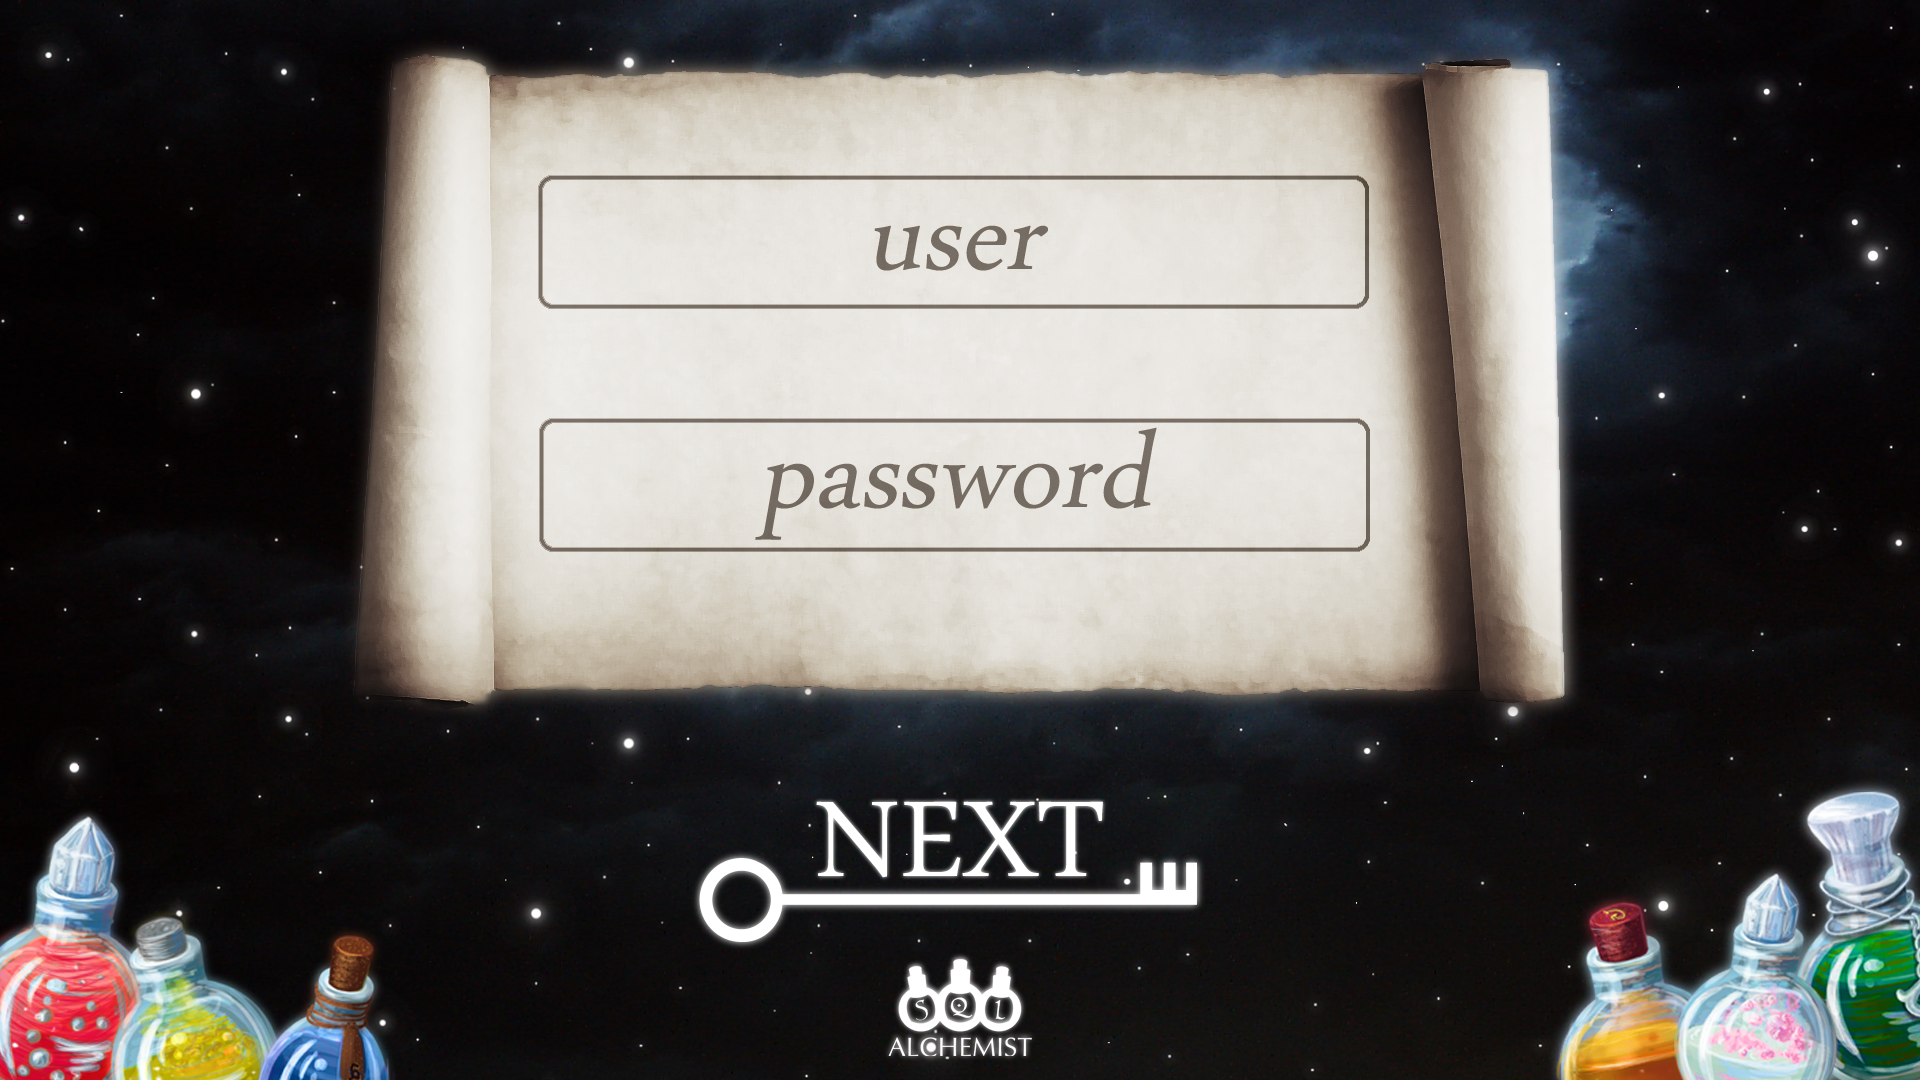
\includegraphics[width=0.7\textwidth]{figures/login_screen.png}
\caption{Login}
\label{gui}
\end{figure}
\end{ui}

\begin{ui}{30}{Minispiel-HUD}
Das Minispiel wird über die Maus gesteuert. Durch Klicks kann der Spielcharakter springen. Durch das Klicken der Potions im linken
unteren Rand des Screens können diese ebenfalls eingesetzt werden.
Durch das Klicken des „Beenden“-Buttons, dargstellt durch ein X, kann das Minispiel befrüht beendet werden.
\end{ui}

\begin{ui}{40}{SQL-Trainer-Screen}
Hier wird es dem User möglich sein, eine Aufgabe zu lösen. Dies geschieht über die Eingabe in ein Textfeld. 
Über einen Button kann das eingegebene Statement auf Korrektheit überprüft werden. Eventuelle Fehlerhinweise
werden ebenfalls in einem Textfeld visualisiert.
\end{ui}

\begin{ui}{20}{Menüführung}
\begin{figure}[ht]
\centering
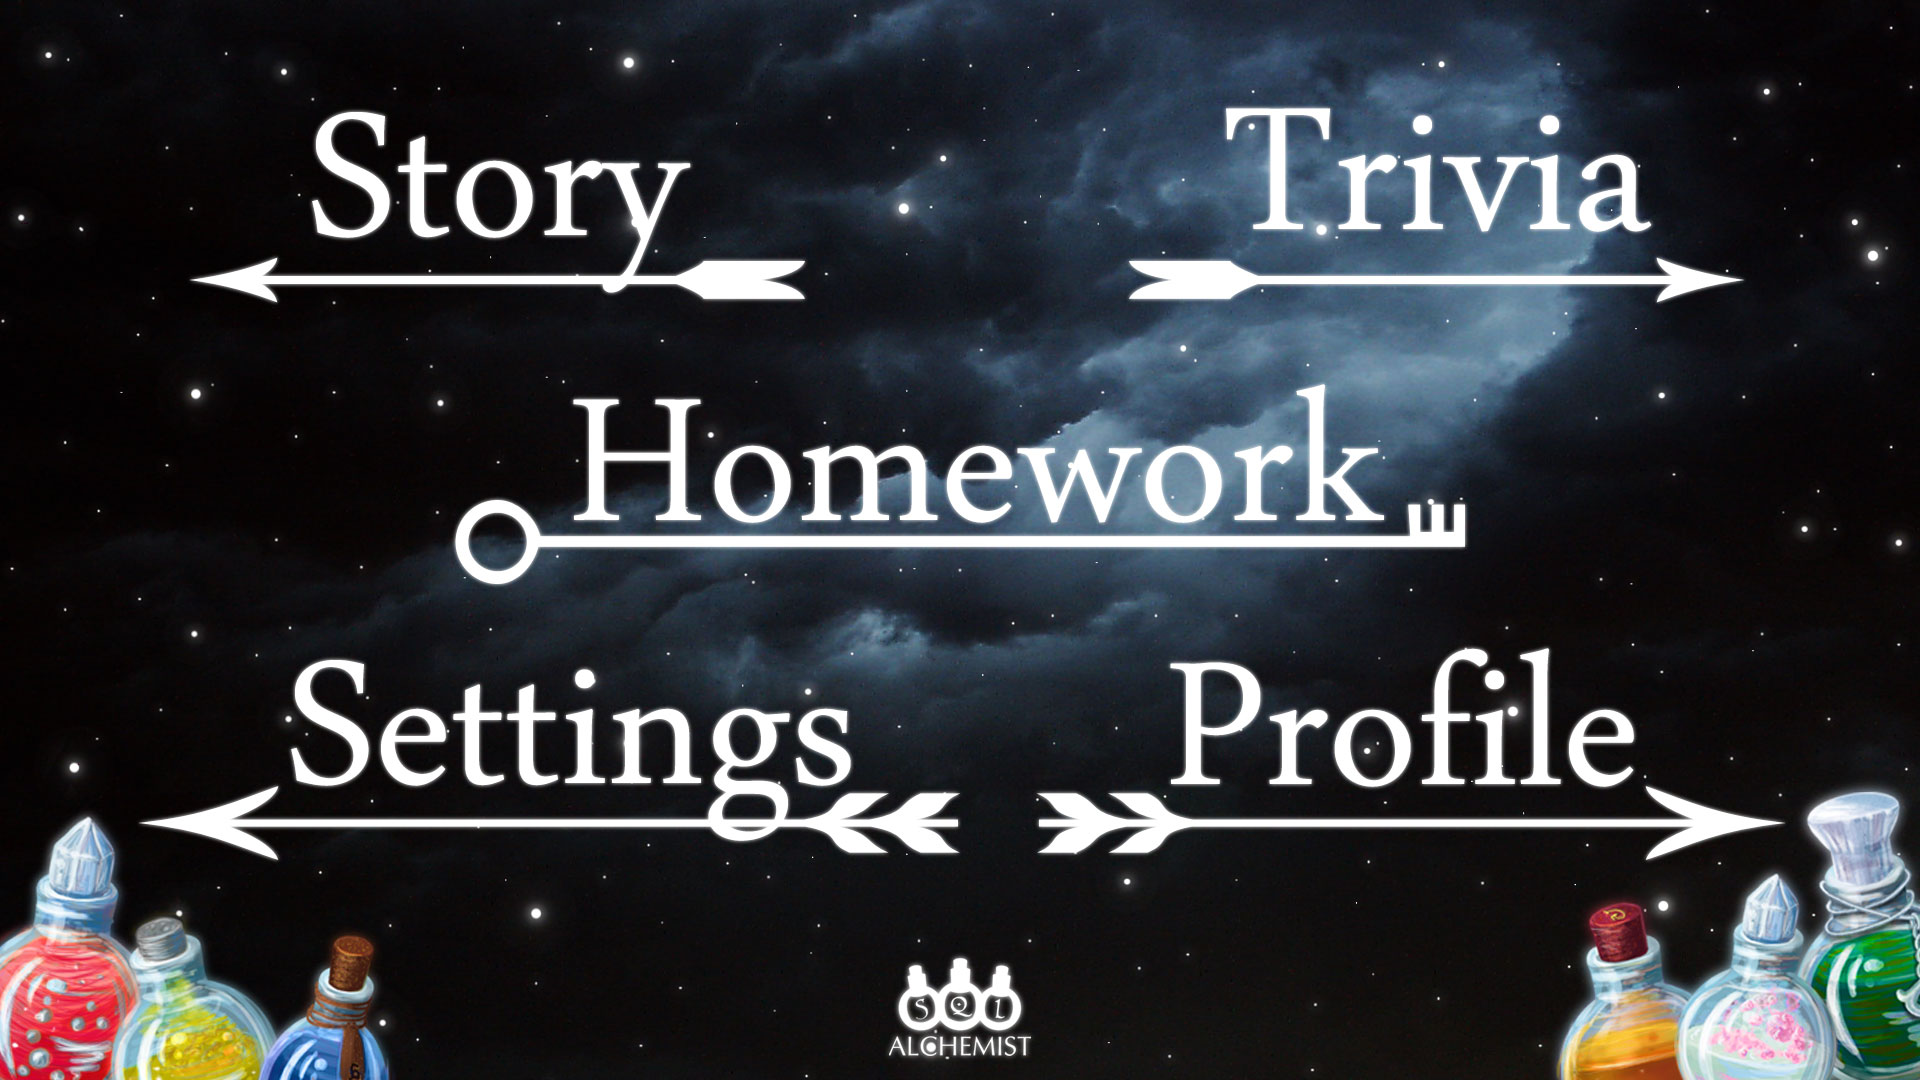
\includegraphics[width=0.7\textwidth]{figures/home_screen.png}
\caption{Men\"uf\"uhrung}
\label{gui}
\end{figure}
Das Hauptmenü ist dass zentrale Userinterface zur Kotrolle des Programmablaufes. 

Hier kann der User über Mauseingaben entweder weitere Teilmenüs 
aufrufen, wie den Trivia-, den Storymodus. Auch die Ranglisten k\"onnen in diesem Men\"u eingesehen werden.
Weiterhin bietet sich den Studenten unter den Usern die Möglichkeit, sich ihren Hausaufgaben zu widmen. Hierf\"ur ist ebenfalls eine eigener Men\"upunkt 
vorgesehen. Au{\ss}erdem gibt es die Möglichkeit sich in das Untermenü der Settings zu begeben, wo der User s\"amtliche Einstellungen ver\"andern kann.
\end{ui}


\begin{ui}{50}{Admin-Tool}
\begin{figure}[ht]
\centering
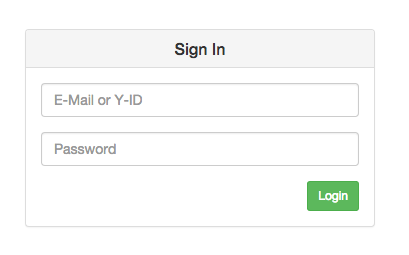
\includegraphics[width=0.7\textwidth]{figures/sign_in_admintool.png}
\caption{Login zum Admin-Tool}
\label{gui}
\end{figure}
Das Admin-Tool ist das zentrale Userinterface zur Kotrolle der User- und Aufgabenverwaltung. Hier kann sich der User einloggen um nachzuschauen ob er die 
Hausaufgaben bestanden hat oder nicht. Des Weiteren kann sich hier der Admin anmelden um Einstellungen zu ver\"andern oder Aufgabenpakete in die Datenbank 
einzupflegen. Jeder bef\"ordete User wird die M\"oglichkeit haben \"uber diesen Login selbst SQL-Aufgaben zu erstellen.   
\end{ui}



